\section{Proposed method}
\label{sec:proposed_method}

In this stage of the research the basic structure of the method to solve the energy issue in the mobile sensing apps has been defined.
The Figure \ref{fig:methodology-stages} shows the workflow of this method.
However, prior to the description of the method elements, it is important to remark the scope of the current research.

\begin{figure}[h]
\centering
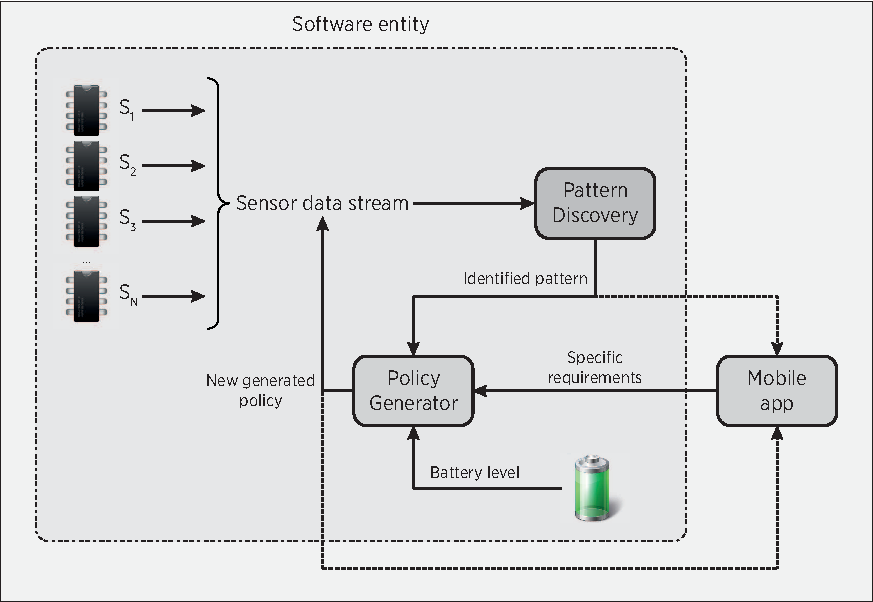
\includegraphics[scale=0.7]{methodology-stages}
\caption[Workflow of the proposed method]{Workflow of the proposed method.}
\label{fig:methodology-stages}
\end{figure}

\subsection{Scope of the research} 
\label{sub:scope_of_the_research}

The work to be performed in this research will be materialized in a software element following:
\begin{itemize}
	\item The pure-software approach.
	\item The individual sensing scale.
	\item The opportunistic paradigm.
\end{itemize}

Additionally, the sensors to be employed are the ones describing motion --- \emph{inertial sensors} --- like GPS and accelerometer, as suggested by the committee in the thesis proposal defence.
The patterns to be identified in data captured from sensors are still to be defined.
Also, these patterns' representation is in process of definition.
However, it is possible to state that a tentative set of patterns can be composed of \emph{no movement}, \emph{walking}, \emph{running}, and \emph{moving in vehicle}.

\subsection{Data acquisition} 
\label{sub:data_acquisition}
As can be seen in Figure \ref{fig:methodology-stages}, the data acquisition is the starting and ending point of the method's workflow.
This component will be in charge of gathering streams of data that will be used later to discover a pattern in user behavior.
It is important to note that this element will be influenced by the feedback information generated by the \emph{Policy generator element}.

\subsection{Pattern identifier element} 
\label{sub:pattern_identifier_element}
This component will receive the sensors data coming from the \emph{Data acquisition} module.
Since this component has to perform data analysis tasks, it should include a memory mechanism for storing and accesing data.
The pattern recognition techniques for identifying relevant events in sensor data are also to be researched, selected and possibly adapted for its execution in a smartphone.

\subsection{Policy generator element} 
\label{sub:policy_generator_element}
This component will create policies based on the pattern identified from sensor data, precision and energy hints provided by mobile app, and current status of physical constraints (battery level) of mobile platform.
Because of this, it is the element that supplies \emph{smartness} to the platform.
The policy created can be implemented by modifying the duty cycling of sensors.

The definition and representation of the policy are also in process of definition.
